\documentclass{article}

\usepackage{graphicx}
\usepackage{xcolor}
\usepackage{pdfpages}
\usepackage[
    a4paper, 
    left=3cm, 
    right=3cm, 
    top=2.5cm, 
    bottom=2.5cm
]{geometry}
\usepackage{hyperref}
\usepackage[T1]{fontenc}


\begin{document}

\begin{titlepage}
	\centering
    % --- Logo --- 
    
\includegraphics[width=\textwidth]{assets/uliege-fsa.png} \\[1 cm]
    % --- Header ---
	\textsc{\Large INFO0004 - Object-Oriented Programming Project} \\[0.4 cm]
    % --- Title ---
	\rule{\linewidth}{0.2 mm} \\[0.4 cm]
	{\Large \bfseries Project Report - Carré Surfer} \\
	\rule{\linewidth}{0.2 mm} \\[1.5 cm]
    % --- Minipage ---
	\begin{minipage}[t]{0.49\textwidth}
		\begin{flushleft} \large
		\textbf{Teacher:} \\
            Laurent MATHY \\[0.5 cm]
            \textbf{Teaching Assistant:} \\
            Elias PIETTE \\
            Gaulthier GAIN \\
            Lev MALCEV
		\end{flushleft}
	\end{minipage}
    \hfill 
	\begin{minipage}[t]{0.49\textwidth}
		\begin{flushright} \large
        \textbf{Author:} \\
            Valérian WISLEZ s200825 
		\end{flushright}
	\end{minipage}
    \vfill	
    \textsc{\Large Academic Year 2025-2026} \\[1.0 cm]	
\end{titlepage}



\section{Introduction}

This report describes the architecture and design choices of an Object-Oriented Programming (OOP) project called "Carré Surfer", written in C++ for the course of Object-Oriented Programming Projects.

Section \ref{sec: features} describes the final game features, including the required extended features. Section \ref{sec: architecture} describes the main OOP mechanisms used and the overall code architecture. Finally, Section \ref{sec: improvements} enumerate a bunch of potential improvements for the game, both in terms of logic and code quality.

\section{Features} \label{sec: features}

We enumerate briefly the game features, focusing on the two extended functionalities that have been asked to implement, namely: the Bus obstacle and the text rendering, which may be seen in Fig. \ref{fig: screenshot}.

\begin{figure}[ht]
    \centering
    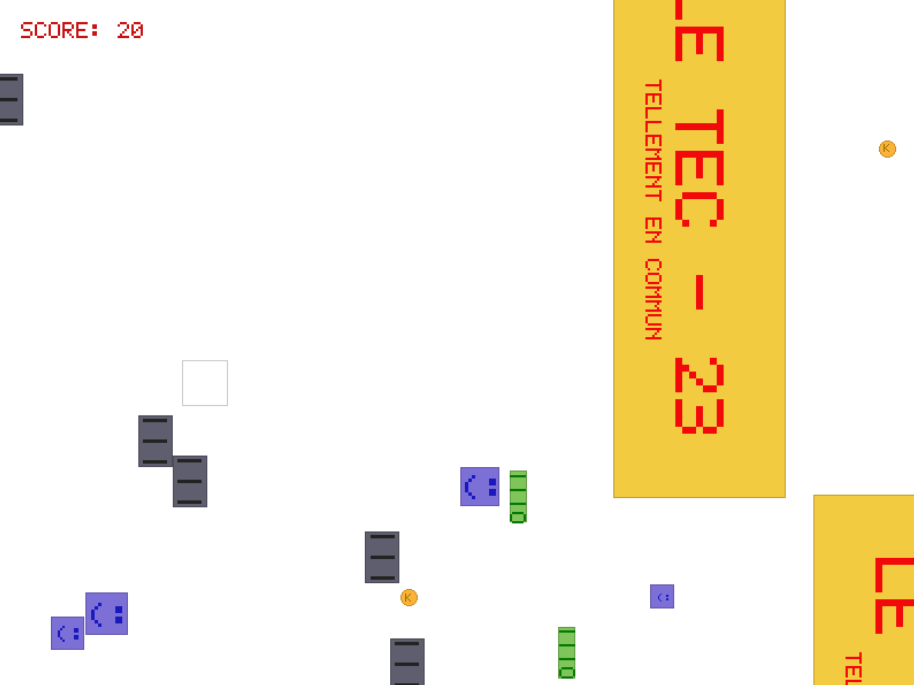
\includegraphics[width=0.8\textwidth]{assets/game_screenshot.png}
    \caption{A typical game screenshot containing all the obstacles types and showing text rendering.}
    \label{fig: screenshot}
\end{figure}

The game's main features include the expected screen-shaking, invincibility, inverted controls, weighted obstacle spawning, as well as custom obstacles-obstacles and player-obstacles collisions.

The \texttt{Bus} is a new dynamic \texttt{Obstacle} featuring randomized vertical speed and acceleration to efficiently block player movement and force it to take another path to avoid obstacles. Meanwhile, the text rendering system is used not only to display real-time game state information like the player's score, but also to support more advanced entity graphics. Indeed, by rendering text overlays directly onto entities, we emulate more complex sprites and thus enhance the visual rendering of obstacles.

\section{Architecture} \label{sec: architecture}

We will now go over the main architecture concepts in the code and motivate them.

\subsection{Classes hierarchy} \label{sec: classes_hierarchy}

You may find the full classes and structs diagram in Section \ref{apx: overview}. There are two main places where inheritance is exploited: 
\begin{itemize}
    \item classes \texttt{Entity}, \texttt{Player}, \texttt{Obstacle} and its subclasses;
    \item classes \texttt{Shape}, \texttt{Circle}, \texttt{Rectangle}.
\end{itemize}

\paragraph{Entity inheritance} \label{sec: entity_inheritance}

The first inheritance tree is straightforward. Each of these components is an actual \texttt{Entity} on the gameboard that shares the need to move and render, thus inheriting \texttt{Entity}'s physics state and logic, as well as \texttt{Entity}'s rendering methods.

Making an \texttt{Obstacle} class itself is justified because it adds a damage component that is shared by all its subclasses. Moreover, it is easier for double dispatching by having a base class that can act as a default case when no explicit \texttt{resolve()} method exists.

\texttt{Player} is an \texttt{Entity} that holds its own state and logic, linked to input handling and invincibility/blinking/reversing timers, so it deserves its own class. \texttt{Obstacle} subclasses all have their own "business logic" hardcoded as \texttt{static constexpr} (shared between every instance), used at construction time by calling \texttt{Obstacle}'s constructor. 

\texttt{DrunkStudent} and \texttt{Bus} require some of their state to be randomized at construction time, which is solved using delegating constructors, to keep a single source of truth and avoid duplicating logic. 

\texttt{Bus::move()} overrides the \texttt{Entity::move()} method to stop when its speed reaches zero (thereby mimicking a Bus that stops near a bus station).

\paragraph{Shape inheritance} \label{sec: shape_inheritance}

The second inheritance tree consists in an abstract base class \texttt{Shape}, which defines virtual methods for drawing itself on the window and colliding with other shapes. Its two concrete subclasses each hold only the parameters strictly necessary to describe their geometry (either a radius, or a width and a height) but don't store any position. 

This is a deliberate separation of concerns from \texttt{Entity}, which owns the position, speed, and acceleration, while \texttt{Shape} only knows how to interpret that position once it is given one. Therefore, \texttt{Shape::draw()} needs a location, passed as a parameter rather than reading it from a member, which keeps the geometric logic in \texttt{geometry.cpp} free of any notion of physics, which is managed exclusively by \texttt{Entity}. \texttt{Entity} itself holds its shape through a \texttt{unique\_ptr<Shape>}, rather than relying on inheritance: an \texttt{Entity} "has a" shape that may change independently of its own identity, rather than "being" one.

Finally, \texttt{Shape} exposes a center\_offset() method used purely for rendering: since \texttt{Rectangle} is drawn from its top-left corner while \texttt{Circle} is drawn from its center, this method is simply overriden by \texttt{Shape}'s subclasses.

\subsection{State management} \label{sec: state_management}
State management follows a consistent pattern across the codebase: data is declared \texttt{constexpr} whenever it is immutable and known at compile time, and \texttt{static} when that data does not need to vary between instances of the same class.

This pattern is most visible in the \texttt{Obstacle} hierarchy, where each subclass defines its own "business logic" members. These values are passed up to \texttt{Obstacle}'s constructor at construction time, so the base class remains agnostic of which concrete obstacle it represents while still enforcing a common interface.

At a higher level, \texttt{Game} owns the overall state of a game session: the frame rate, board dimensions, and ownership of the active obstacles. Rather than exposing this state directly, \texttt{Game}'s control flow is split into small private methods, so that \texttt{main()} and the class's only public entry point, \texttt{Game::run()}, stay minimal and readable. Resetting a game session follows the same delegation principle used elsewhere in the project: \texttt{Game} does not reset every object's internal fields itself but simply clears what it directly owns and calls into each owned object's own reset method, letting each class remain responsible for its own state.

\subsection{Double-dispatch} \label{sec: double_dispatch}

A recurring problem in the project is choosing the correct behavior to execute based on the dynamic types of two objects rather than a single one. A regular virtual method call only dispatches on the dynamic type of the object it is called on. When both operands of an operation can vary independently, as is the case for two colliding \texttt{Shapes}, or two colliding \texttt{Entity}s, a single virtual call is not enough to select the right implementation. This is the classical motivation for double dispatch: a first virtual call resolves the dynamic type of the first object, which in turn issues a second virtual call on the other object. Only after both calls have taken place is the concrete pair of types known, and the right function can be selected. This technique is notably used in compiler design, e.g. to implement the Visitor pattern over an abstract syntax tree, which is what originally motivated its use here.

The project uses this mechanism in two distinct places: geometric collision detection between \texttt{Shapes}, and collision resolution between \texttt{Entity}s (both \texttt{Obstacle} - \texttt{Obstacle} and \texttt{Player} - \texttt{Obstacle}).

\paragraph{Geometry collisions} 

Since \texttt{Summoner} spawns \texttt{Obstacle}s at random positions on the right side of the board and they may collide with each other, which would make the obstacles overlap, we deemed necessary to find a way to separate them. We did not want to approximate a circle by an Axis-Aligned Bounding Box (AABB) but instead have faithful collision mechanics.

Because each pair of concrete shapes maps to a distinct geometric test (\texttt{Circle\_vs\_Circle()}, \texttt{Circle\_vs\_AABB()}, \texttt{AABB\_vs\_AABB()}), the right test needs to be selected at runtime based on the two concrete shapes that are actually colliding. 

This is resolved through \texttt{Shape::collide\_with()}, which dispatches on the dynamic type of the shape it is called on and calls either \texttt{collide\_with\_circle()} or \texttt{collide\_with\_rectangle()} on the other shape, resolving the second dynamic type and thereby finding the right shapes combination. 

The geometric tests themselves are implemented as free functions in the geometry namespace rather than as \texttt{Shape} methods, since they operate purely on geometric primitives (center, radius, width/height) and therefore do not belong to either concrete class.

\paragraph{Obstacle collisions} The same mechanism governs gameplay-level collisions, where the goal is to select the appropriate behavior based on the concrete types of the two colliding entities (which may be two Obstacles, or a Player and an Obstacle). 

This is implemented via the \texttt{FirstEntityVisitor} and \texttt{SecondEntityVisitor} classes, which resolve the two dynamic types in turn and ultimately call one of the \texttt{resolve()} free functions. These functions are declared as free functions, rather than as members of any one \texttt{Entity} subclass, since a given interaction between two classes (e.g., a \texttt{Bus} and a \texttt{Obstacle}) does not conceptually belong to either class alone.

To avoid duplicating logic for symmetric interactions (a \texttt{Bus} colliding with a \texttt{DrunkStudent} should behave identically as a \texttt{DrunkStudent} colliding with a \texttt{Bus}), \texttt{resolve()} overloads are written in alphabetical order of their argument types: the first overload matching the alphabetical order implements the actual logic (e.g., \texttt{resolve(Bus, Obstacle)} - that is, a \texttt{Bus} collided an \texttt{Obstacle}), while the "mirror" overload, matching the reversed order (e.g., \texttt{resolve(Obstacle, Bus)} - that is, an \texttt{Obstacle} collided a \texttt{Bus}), simply calls back the first one with its arguments flipped via a small \texttt{flip()} helper. 
This helper mostly serves to flip the direction of the Minimum Translation Vector (MTV) that represents the translation we should apply to the entities to separate them. The referential is relative to which obstacle collides which one, therefore we need to reverse directions.

This convention guarantees there is exactly one place where the logic for a given pair of types is implemented, at the cost of a small maintenance burden: the convention must be respected by hand when adding a new pair, and a missing or inconsistent mirror overload would be a silent source of bugs.

When no dedicated \texttt{resolve()} overload exists for a given pair of concrete types, the mechanism falls back on the inheritance hierarchy described in Section \ref{sec: classes_hierarchy}: a more generic overload of the function is selected. This allows to write only the \texttt{resove()} methods that actually implement a dedicated behavior, instead of having to write every possible combination. For example, there is no \texttt{resolve(Scooter, Player)} combination since \texttt{Scooter} behaves exactly like any other \texttt{Obstacle} (see \ref{sec: improvements} for an idea of improvement). The most generic overload corresponds to two \texttt{Entity}s and simply separates them by splitting their minimum translation vector 50/50, assuring a default case.

\subsection{Memory management and data structures} \label{sec: memory_management}

Memory management in the project completely avoids manual new/delete calls and the associated risk of leaks or dangling references. Most of the variables are located on the stack, but we will detail the places were we have used smart pointers.

\paragraph{Shape ownership} As discussed in \ref{sec: architecture}, an \texttt{Entity} "has a" Shape rather than "being" one, which is expressed through a \texttt{unique\_ptr<Shape>} member. 

Since \texttt{Shape} is an abstract polymorphic type, it cannot be stored by value; a pointer is required to allow an \texttt{Entity} to hold either a \texttt{Circle} or a \texttt{Rectangle} behind the same interface. 

\texttt{unique\_ptr} was preferred over \texttt{shared\_ptr} because the ownership relationship is strictly exclusive: no other object ever needs to share or outlive the \texttt{Shape} beyond its owning \texttt{Entity}'s lifetime, so a \texttt{unique\_ptr} lets the compiler enforce it, while also handling destruction automatically when the \texttt{Entity} itself is destroyed.

\paragraph{Obstacle ownership transfer} 
Obstacles follow a similar pattern. \texttt{Summoner} is responsible for deciding when and which \texttt{Obstacle} to spawn, but it should not hold on to it once it has spawned. Newly created obstacles are therefore returned from \texttt{Summoner} as \texttt{unique\_ptr<Obstacle>} and their ownership is transferred into \texttt{Game}'s own \texttt{vector<unique\_ptr<Entity>>} (which also stores the \texttt{Player}). This also means Game can freely erase an obstacle from its vector (for instance once it goes past the left-hand side of the board, or it is destroyed in a \texttt{Bus} collision) without needing to coordinate with any other part of the code.

\paragraph{Weighted spawning} Moreover, to decide which \texttt{Obstacle} subclass to spawn next, \texttt{Summoner} combines a \texttt{std::discrete\_distribution} with a small factory table: a vector of functions each responsible for constructing one obstacle type and returning it as a \texttt{unique\_ptr<Obstacle>}. 

The \texttt{discrete\_distribution} is configured with the relative spawn weights of each obstacle type and is used to draw an index at random, which is then used to invoke the corresponding factory function. This keeps the spawning logic easy to extend, since adding a new obstacle type only requires appending one weight and one factory function to their respective tables, not touching the spawning mechanism itself.

\section{Improvements} \label{sec: improvements}

During testing, we identified several places where the game could be improved, both in terms of features and realism, as well as coding practice.

\begin{itemize}
    \item Rather than blocking the player on collision, the \texttt{Scooter} could make the player trip, for more varied behavior. This would be easy to add thanks to the double-dispatch visitor already in place.
    \item Introduce namespaces to separate geometry, game logic, and rendering, extending the idea behind \texttt{gfx}.
    \item Make \texttt{scale\_brightness} a method of Color.
    \item \texttt{Vector2D} could arguably be a Shape subclass implementing a \texttt{draw()} method that calls \texttt{drawLine()}. This wasn't needed for the current gameplay, so it wasn't implemented.
    \item \texttt{Summoner}'s spawn rate should scale with the board's vertical size. A private delegating constructor with a linearly tuned coefficient would achieve this.
    \item Use \texttt{std::optional} instead of a nullable pointer for \texttt{Summoner::update()}.
    \item Tighten include directives to strictly what each \texttt{.cpp} file needs, rather than relying on including headers, including themselves other headers, thereby speeding up compilation.
    \item The collision system could be improved: \texttt{Kebab} obstacles can shake when another obstacle spawns inside them, and visual glitches occasionally occur when a \texttt{Kebab} collides with a rectangular obstacle. These were judged out of scope for the project but would be worth fixing. Similarly, two colliding \texttt{Bus}es obstacles should take the minimum of their speed and acceleration rather than one pushing the other. This only requires extending \texttt{CollisionInfo} with this information, which is straightforward.
\end{itemize}

\section{Conclusion} \label{sec: conclusion}

Throughout the project, we have tried to keep concerns strictly separated (physics and identity in \texttt{Entity}, geometry in \texttt{Shape}, rendering left to the main loop) and relied consistently on double dispatch, both for geometry collisions and for entity-to-entity gameplay resolution, rather than falling back on manual type-checking. This consistency was as much a design goal as a practical one: it kept each class focused on a single responsibility and made the codebase easier to extend as new obstacle types were added.

Finally, we tried to make the game as enjoyable to play as possible and we can confirm, from our own testing, that it was.

\appendix{}

\section{AI usage} \label{apx: ai_usage}

AI has been used for this project in the following manner. Google's Gemini (Fast) model was used for correcting spelling and grammar of this report.

We have used Anthropic's Claude (5.2 Sonnet) for helping with geometrical computations both in \texttt{geometry.hpp/.cpp} and in \texttt{text.cpp/.hpp}. Indeed, while the interfaces and concepts are our own thoughts, it was easier to ask an AI to verify or perform the pixels computations because these places are a source of arithmetic bugs (e.g., missing a \texttt{+1}, challenging \texttt{Direction}-based arithmetics and corrections) that would have been too costly to fix in terms of timing. Moreover, we have used this same AI model to discuss about architectures for the project, reflect on our thoughts and dig into C++ and OOP concepts. Google's Gemini (Fast) was also used to explain some unknow concepts and debug some strange compiler messages.

\section{Classes Overview} \label{apx: overview}

You may find hereafter the full classes and structs overview of the project.

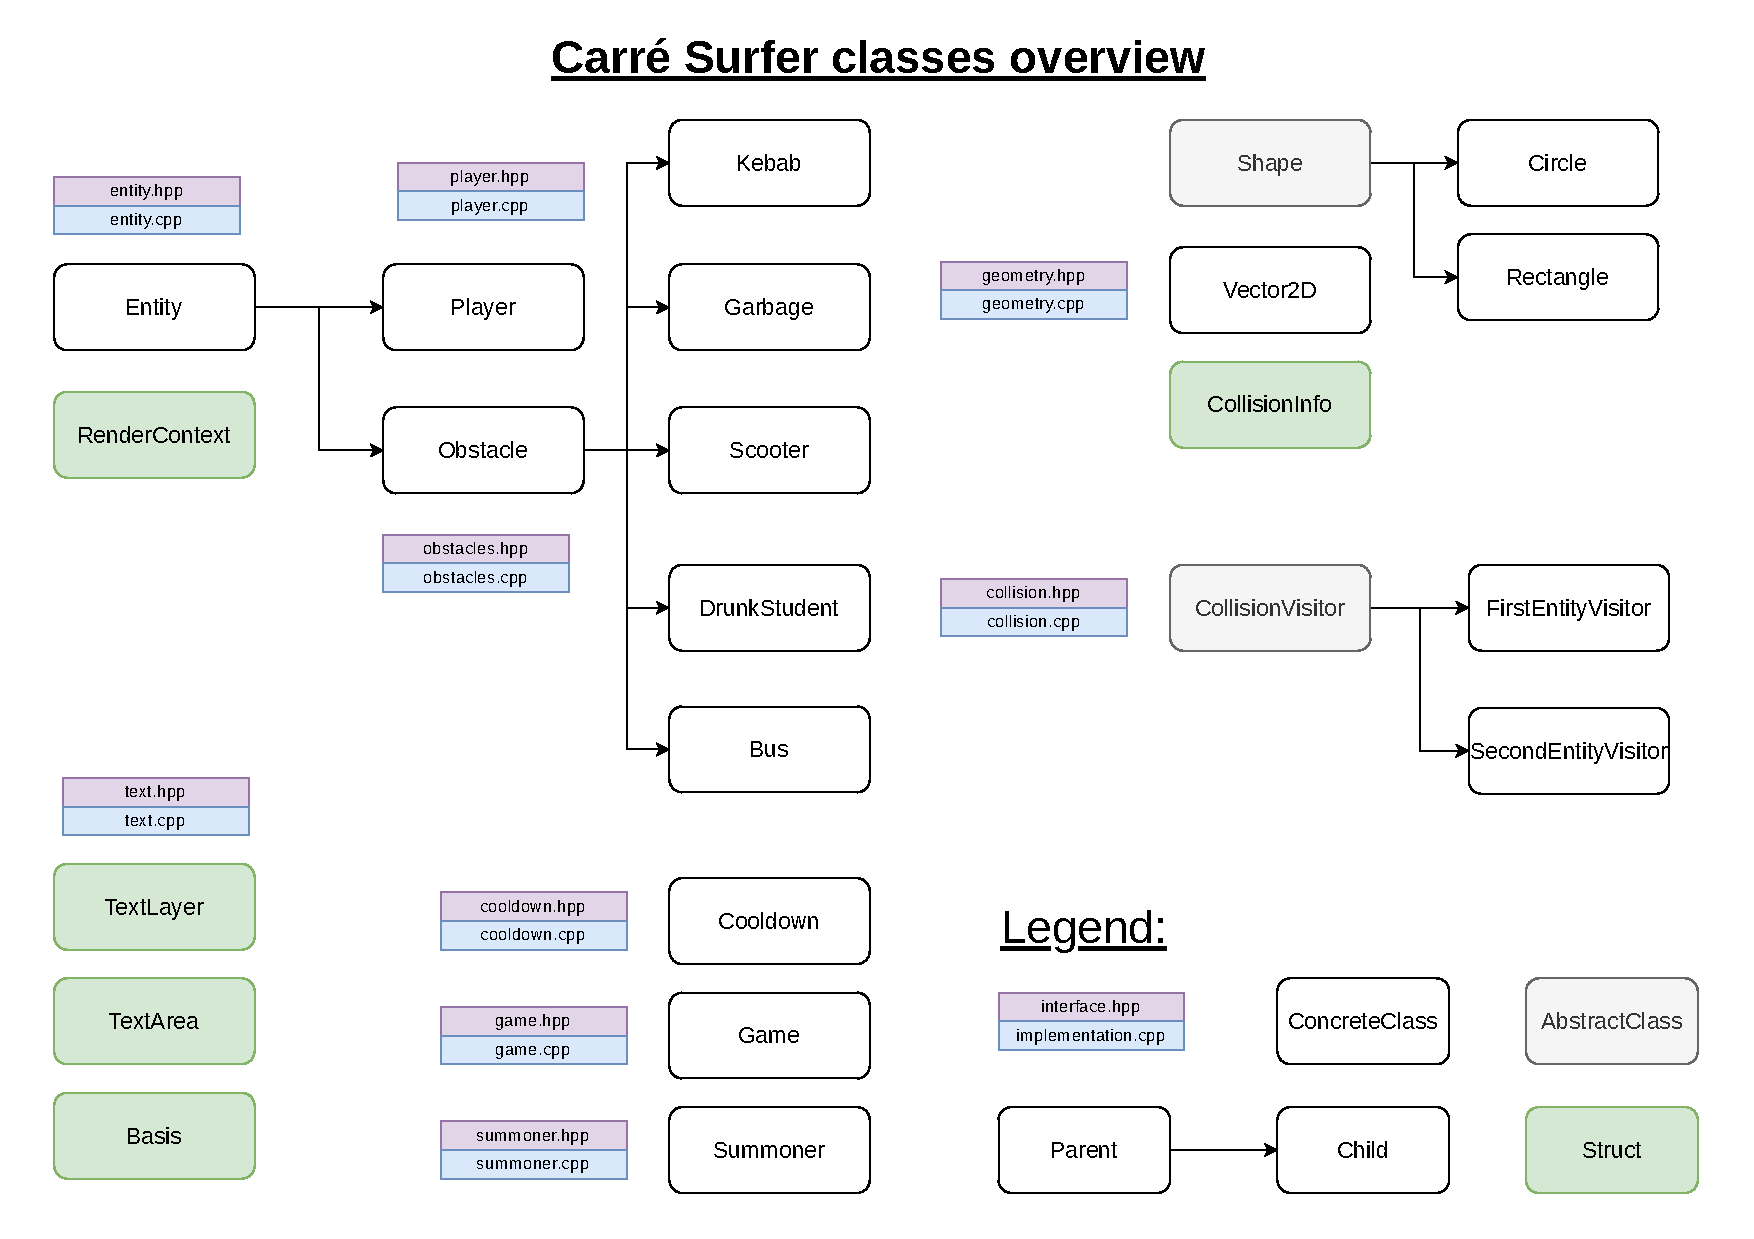
\includepdf[
    pages={1},
    landscape=true,
    pagecommand={\thispagestyle{plain}}
]{assets/overview.drawio.pdf}

\end{document}